\newpage
\section[Functions of Several Variables]{\hyperlink{toc}{Functions of Several Variables}}

\subsection{Banach Fixed Point Theorem}
\noindent Our goal in this chapter will be to work up to the Inverse Function Theorem. This chapter in Rudin begins by covering the necessary results in linear algebra; we will assume this has been covered in a prior course, so we will omit discussion of items 9.1-9.9. However, these can be read for a refresher of the material.

We will start off this chapter with discussion of the Banach fixed point theorem (also known as the Contraction principle), as it is independent of the rest of the chapter's content. It will be used in the proof of the inverse function theorem, but also applies in a more general setting.

\setcounter{rudin}{21}

\begin{definition}{Contractions}{9.22}
    Let $(X, d)$ be a metric space. Suppose there exists $c < 1$ such that the map $\phi: X \mapsto X$ satisfies $d(\phi(x), \phi(y)) \leq cd(x, y)$ for all $x, y \in X$ (that is, the images of $x, y$ are closer by a factor $c$ compared to the original $x, y$). Then, we call $\phi$ a \textbf{contraction} of $X$ into $X$.
\end{definition}
\begin{nlemma}{}{}
    Every contraction $\phi: X \mapsto X$ is uniformly continuous.
\end{nlemma}
\begin{nproof}
    Take $\delta = \frac{\e}{c}$ in the definition of uniform continuity. \qed
\end{nproof}

\begin{theorem}{Banach Fixed Point Theorem/Contraction Mapping Theorem}{9.23}
    Let $(X, d)$ be a complete metric space, and suppose $\phi: X \mapsto X$ is a contraction. Then, there exists a unique $x \in X$ such that $\phi(x) = x$. We call this x a \emph{fixed point}. 
\end{theorem}
\noindent The proof of the above theorem gives an algorithm to find $x$ which converges exponentially fast.

\begin{figure}[htbp]
    \centering
    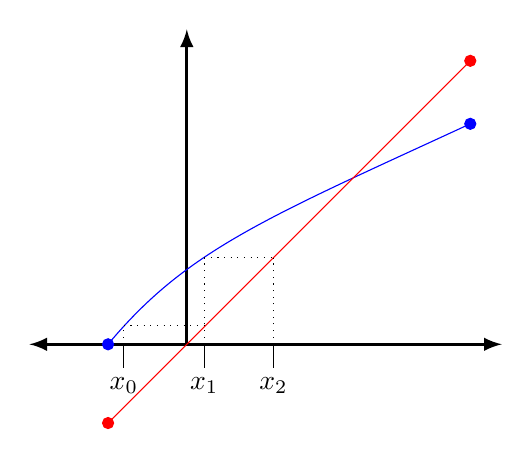
\begin{tikzpicture}[scale=2]
        \draw[-latex, very thick] (0, 0) -- (2, 0);
        \draw[-latex, very thick] (0, 0) -- (0, 2);
        \draw[-latex, very thick] (0, 0) -- (-1, 0);
        \draw[blue] (-0.5, 0) .. controls (0, 0.6) and (0.5, 0.8 ).. (1.8, 1.4);
        \draw[fill = blue, draw = blue] (-0.5, 0) circle (1pt);
        \draw[fill = blue, draw = blue] (1.8, 1.4) circle (1pt);
        \draw[red] (-0.5, -0.5) -- (1.8, 1.8);
        \draw[fill = red, draw = red] (-0.5, -0.5) circle (1pt);
        \draw[fill = red, draw = red] (1.8, 1.8) circle (1pt);
        \draw[] (-0.4, 0) -- (-0.4, -0.15);
        \node[below] at (-0.4, -0.15) {$x_0$};
        \draw[dotted] (-0.4, 0) -- (-0.4, 0.12);
        \draw[dotted] (-0.4, 0.12) -- (0.13, 0.12);
        \draw[dotted] (0.11, 0) -- (0.11, 0.55);
        \draw[] (0.11, 0) -- (0.11, -0.15);
        \node[below] at (0.11, -0.15) {$x_1$};
        \draw[dotted] (0.11, 0.55) -- (0.55, 0.55);
        \draw[dotted] (0.55, 0) -- (0.55, 0.55);
        \draw[] (0.55, 0) -- (0.55, -0.15);
        \node[below] at (0.55, -0.15) {$x_2$};
    \end{tikzpicture}

    \caption{Visualization of the algorithm for finding the fixed point $x$ in Theorem \ref{thm:9.23} for the case where $X = \RR$. The fact that $\phi$ is a contraction makes it such that it has slope less than $1$. The fixed point is the point of intersection between $y = x$ and $y = \phi(x)$. The iterative algorithm sketched above gives an exponentially fast way of finding this point of intersection, by iteratively applying $\phi$ to the initial guess $x_0$.}
    \label{fig59}
\end{figure}

\begin{nproof}
    We first show uniqueness. If $\phi(x) = x$ and $\phi(y) = y$, then $d(\phi(x), \phi(y)) \leq cd(x, y)$. But since $c < 1$, $d(x, y) \leq cd(x, y)$ is only satisfied if $d(x, y) = 0$. Hence, $x = y$ and the fixed point is unique.

    We next show existence. Given $x_0 \in X$, let $x_1 = \phi(x_0)$, $x_2 = \phi(x_1) = \phi\circ \phi(x_0)$, $x_3 = \phi(x_2) = \phi\circ\phi\circ\phi(x_0)$ and so on, with $x_{n+1} = \phi(x_n) = \phi \circ \ldots \circ \phi(x_0)$ with the composition carried out $n+1$ times. The goal is to show this sequence is Cauchy, and has a limit which is a fixed point. We then have that $d(x_{n+1}, x_{n+2}) = d(\phi(x_n), \phi(x_{n+1})) \leq cd(x_{n+1}, x_n)$, so by induction, it follows that $d(x_{n+1}, x_n) \leq c^nd(x_1, x_0)$. Hence, for $n > m$ we have that:
    \begin{align*}
        d(x_n, x_m) &\leq \sum_{i=m+1}^n d(x_i, x_{i-1}) & \text{(Triangle Inequality)}
        \\ &\leq \sum_{i=m+1}^n c^{i-1}d(x_1, x_0)
        \\ &\leq \sum_{i=m+1}^\infty c^{i-1}d(x_1, x_0)
        \\ &= \frac{c^m}{1-c}d(x_1, x_0) & \text{(Convergent Geometric Series)}
    \end{align*}
    $c^m$ can be as small as we like by taking sufficiently large $m$, so $\set{x_n}$ is Cauchy, and by the completeness of $X$, $x_n \rightarrow x$ for some $x$. Since $\phi$ is a contraction, it is (uniformly) continuous by the above Lemma, and since $x_n \rightarrow x$, we have that $\phi(x_n) \rightarrow \phi(x)$, and hence:
    \begin{align*}
        \phi(x) = \linf \phi(x_n) = \linf x_{n+1} = x.
    \end{align*}
    This shows that $x$ is the desired fixed point. \qed
\end{nproof}

\subsection{Differentiation of Functions of Several Variables}
\noindent In this section we discuss the differentiation of functions $f: \RR^n \mapsto \RR^m$. It will be instructive to remind ourselves of the familiar case of $n = m = 1$. In this case, we defined the derivative as:
\begin{align*}
    f'(x) = \lim_{h \rightarrow 0}\frac{f(x + h) - f(x)}{h}
\end{align*}
where we would say $f$ was differentiable at $x$ if the above limit existed. We want to now try to generalize this notion to higher dimensions. It obviously does not apply directly, as in this general setting, $\v{f}(\v{x} + \v{h}) - \v{f}(\v{x})$ is a vector in $\RR^m$ and $\v{h}$ is a vector in $\RR^n$, and the division of such vectors is not well defined. Let us try to recast the $n = m = 1$ derivative into a form that lends itself better to generalization. We could equivalently write the above derivative expression as:
\begin{align*}
    \lim_{h \rightarrow 0}\frac{f(x + h) - f(x) - f'(x)h}{h} = 0
\end{align*}
and hence:
\begin{align*}
    \lim_{h \rightarrow 0}\abs{\frac{f(x + h) - f(x) - f'(x)h}{h}} = 0.
\end{align*}
Equivalently, we can say that $f(x + h) = f(x) + f'(x)h + r(h)$ with $\lim_{h \rightarrow \infty}\frac{r(h)}{h} = 0$; $r(h)$ is then the ``remainder term''. With this interpretation, $f'(x)h$ is the best linear approximation to $f(x + h) - f(x)$. This last characterization makes sense for general vectors in $\RR^k$, so let us define derivatives with this notion!

\setcounter{rudin}{10}

\begin{definition}{Derivatives of $f: \RR^n \mapsto \RR^n$}{9.11}
    Let $m, n \in \NN$ and $E \subset \RR^n$ be open. Define a function $\v{f}$ such that $\v{f}: E \mapsto \RR^m$, and let $\v{x} \in E$. We say that $f$ is \textbf{differentiable} at $\v{x}$ and has \textbf{derivative} $A \in L(\RR^n, \RR^m)$ ($\v{f}'(\v{x}) = A$) if:
    \begin{align*}
        \lim_{\v{h} \rightarrow \v{0}} \frac{\abs{\v{f}(\v{x} + \v{h}) - \v{f}(\v{x}) - A\v{h}}}{\abs{\v{h}}} = 0
    \end{align*}
\end{definition}
\noindent Note that the $\abs{}$ in the above definition refer to the $L_2$/Euclidean norm of $\RR^m$ (in the numerator) and $\RR^m$ (in the denominator) respectively. Furthermore, observe that $A$ is not just a number (as it is in the linear case) but an \emph{linear transformation} such that $A \in L(\RR^n, \RR^m)$, where $L(\RR^n, \RR^m)$ is the vector space of linear maps from $\RR^n$ to $\RR^m$. Equivalently, the above definition can be phrased as:
\begin{align*}
    \v{f}(\v{x} + \v{h}) = \v{f}(\v{x}) + A\v{h} + \v{r}(\v{h}) \text{ with } \lim_{\v{h} \rightarrow \v{0}} \frac{\abs{\v{r}(\v{h})}}{\abs{\v{h}}} = 0
\end{align*}
where again, $A\v{h}$ is the ``best linear approximation'' to $\v{f}(\v{x} + \v{h}) - \v{f}(\v{x})$. 

\begin{theorem}{Uniqueness of Higher Dimensional Derivatives}{9.12}
    The derivative $A$ defined above is unique.
\end{theorem}
\begin{nproof}
    Suppose $\v{f}(\v{x} + \v{h}) = \v{f}(\v{x}) + A_1\v{h} + \v{r}_1(\v{h})$ and $\v{f}(\v{x} + \v{h}) = \v{f}(\v{x}) + A_2\v{h} + \v{r}_2(\v{h})$ with $\v{r}_1(\v{h}) \in O(\v{h})$ and $\v{r}_2(\v{h}) \in O(\v{h})$. Let $B = A_1 - A_2$. Then, $0 = (A_1 - A_2)\v{h} + (\v{r}_1 - \v{r}_2)$. Therefore, $B\v{h} = \v{r}_2 - \v{r}_1$, so for $\v{h} \neq \v{0}$ and scalar $t \neq 0$ we have that:
    \begin{align*}
        \frac{\abs{B\v{h}}}{\abs{\v{h}}} = \frac{\abs{B(t\v{h})}}{\abs{t\v{h}}} \leq \frac{\abs{\v{r}_1(t\v{h})}}{\abs{t\v{h}}} + \frac{\abs{\v{r}_2(t\v{h})}}{\abs{t\v{h}}} \quad \text{(Triangle Inequality)}
    \end{align*} 
    Letting $t$ go to zero, we have that the RHS goes to zero. Hence, $\frac{\abs{B\v{h}}}{\abs{\v{h}}} \rightarrow 0$. But $\frac{\abs{B\v{h}}}{\abs{\v{h}}}$ is independent of $t$, so it must be zero. Hence, $B$ is the zero map and hence $A_1 = A_2$. We conclude that the derivative $A$ is unique. \qed
\end{nproof}

\noindent Note that if $f'(x)$ exists for all $x$ in $E$, then we can regard $\v{f}'$ as a function $\v{f}': E \mapsto L(\RR^n, \RR^m)$. Let us clarify that $\v{f}'$ is \emph{not} a vector valued function, but a linear map; we use the notation $\v{f}'$ to denote it as the derivative of a vector valued function.

\setcounter{rudin}{13}
\begin{example}{}{9.14}
    Suppose $f: \RR^n \mapsto \RR^m$ is linear. Then:
    \begin{align*}
        \v{f}(\v{x} + \v{h}) = \v{f}(\v{x}) + \v{f}(\v{h}) + 0
    \end{align*}
    for all $\v{x}, \v{h} \in \RR^n$. Hence, $\v{f}'(x) = \v{f}$ for all $\v{x}, \v{h} \in \RR^n$. The derivative is the function itself (\emph{not} the value $\v{f}(\v{x})$) when $\v{f}$ is linear.

    Note that for $n = m = 1$, we can identify a linear map $f: \RR \mapsto \RR$ as $f(x) = \alpha x$, with $\alpha \in \RR$. Then, $f'(x) = \alpha$ is consistent with the above general result.
\end{example}
\begin{ntheorem}{}{}
    If $\v{f}'(\v{x})$ exists, then $\v{f}$ is continuous at $\v{x}$.
\end{ntheorem}
\begin{nproof}
    $\lim_{\v{h} \rightarrow 0}\v{f}(\v{x} + \v{h}) = \lim_{\v{h} \rightarrow 0}\left(\v{f}(x) + \v{f}'(x)\v{h} + O(\v{h})\right) = \v{f}(x)$.
\end{nproof}

\begin{ndef}{: Norm of a linear map}{}
    Let $A: \RR^n \mapsto \RR^m$ be a linear map. We then define:
    \begin{align*}
        \norm{A} = \sup\set{\abs{A\v{x}}: \abs{\v{x}} \leq 1}.
    \end{align*}
\end{ndef}
\noindent In other words, we have that $\abs{A\v{x}} = \abs{A\frac{\v{x}}{\abs{\v{x}}}}\abs{\v{x}} \leq \norm{A}\v{x}$ for all $\v{x} \in \RR^n$. $\norm{A}$ is the best constant bound. Before moving onto the next theorem, we note a couple facts about $\norm{A}$:
\begin{enumerate}
    \item $\norm{A} < \infty$ for any linear map $A$.
    \item $\norm{AB} \leq \norm{A}\norm{B}$.
    \item $d(A, B) = \norm{A - B}$, which defines a metric on the space of linear maps.
\end{enumerate}

\begin{theorem}{Chain Rule}{9.15}
    Suppose that $E \subset \RR^n$, $E$ is open, and $\v{f}: E \mapsto \RR^m$. Furthermore, suppose $V \subset \RR^m$ is open and $\v{f}(E) \subset V$. Define $\v{g}: V \mapsto \RR^k$, and suppose $\v{f}'(\v{x}_0)$ exists and $\v{g}'(\v{f}'(\v{x}_0))$ exists for some $\v{x}_0 \in E$. Let $\v{F} = \v{g} \circ \v{f}: E \mapsto \RR^k$. Then, we have that $\v{F}'(\v{x}_0)$ exists, and $\v{F}'(\v{x}_0) = \v{g}'(\v{f}(\v{x}_0))\v{f}'(\v{x}_0) \in L(\RR^n, \RR^k)$.
\end{theorem}
\noindent As a point of clarification, note that $\v{g}'(f(\v{x}_0))\v{f}'(\v{x}_0)$ denotes a composition of linear operators, where $\v{f}': \in L(\RR^n, \RR^m)$ and $\v{g}' \in L(\RR^m, \RR^k)$.
\begin{figure}[htbp]
    \centering
    \begin{tikzpicture}[scale=2.5]
        \draw[] (0, 0) -- (1, 0) -- (1, 1) -- (0, 1) -- (0, 0);
        \draw[draw= white, fill = white!60!black, fill opacity = 0.3] (3, 0.25) -- (3, 1) -- (2, 1) -- (2, 0.25) -- (3, 0.25);
        \draw[] (2, 0) -- (3, 0) -- (3, 1) -- (2, 1) -- (2, 0);
        \draw[] (4, 0) -- (5, 0) -- (5, 1) -- (4, 1) -- (4, 0);
        \draw[->, thick] (1.1, 0.75) -- (1.9, 0.75);
        \draw[->, thick] (3.1, 0.75) -- (3.9, 0.75);
        \draw[->, thick] (1.1, -0.1) .. controls (2.5, -0.5) .. (3.9, -0.1);
        \draw[dotted, fill = white!60!black, fill opacity=0.3] (0.5, 0.5) circle (10pt);
        \draw[dotted] (2, 0.25) -- (3, 0.25);
        \draw[dotted, fill = white!60!black, fill opacity=0.3] (2.6, 0.6) circle (8pt);
        \node[right] at (0, 0.15) {$\RR^n$};
        \node[right] at (2, 0.15) {$\RR^m$};
        \node[right] at (4, 0.15) {$\RR^k$};
        \node[right] at (2, 0.35) {$V$};
        \node[] at (0.32, 0.32) {$E$};
        \node[] at (2.55, 0.45) {$\v{f}(E)$};
        \node[above] at (1.5, 0.75) {$\v{f}$};
        \node[above] at (3.5, 0.75) {$\v{g}$};
        \node[above] at (2.5, -0.4) {$\v{F}$};
        \filldraw[] (0.4, 0.6) circle (0.5pt);
        \node[above] at (0.4, 0.6) {$\v{x}_0$};
        \filldraw[] (2.65, 0.6) circle (0.5pt);
        \node[above] at (2.65, 0.6) {$\v{f}(\v{x}_0)$};
    \end{tikzpicture}
    \caption{Visualization of the sets and functions in Theorem \ref{thm:9.15}.}
    \label{fig60}
\end{figure}
\begin{nproof}
    The proof is very similar to the one dimensional case. We observe that:
    \begin{align*}
        \v{F}(\v{x}_0 + \v{h}) - \v{F}(\v{x}_0) &= \v{g}(\v{f}(\v{x}_0 + \v{h})) - \v{g}(\v{f}(\v{x}_0)).
    \end{align*}
    We can then write $\v{f}(\v{x}_0 + \v{h})$ as $\v{f}(\v{x}_0) + \v{K}$ where $\v{K} = \v{f}'(\v{x}_0)\v{h} + \v{u}(\v{h})$ with $\v{u}(\v{h}) \in O(\v{h})$. We can then write:
    \begin{align*}
        \v{F}(\v{x}_0 + \v{h}) - \v{F}(\v{x}_0) &= \v{g}'(\v{f}(\v{x}_0))\v{K} + \v{V}(\v{K})
        \\ &= \v{g}'(\v{f}(x_0))\left[\v{f}'(x_0)\v{h} + \v{u}(\v{h})\right] + \v{V}(\v{K})
        \\ &= \v{g}'(\v{f}(x_0))\v{f}'(x_0)\v{h} + \v{g}'(\v{f}(x_0))\v{u}(\v{h}) + \v{V}(\v{K})
    \end{align*} 
    where $\v{g}'(\v{f}(x_0))\v{u}(\v{h}) + \v{V}(\v{K}) = \v{r}(\v{h})$ is our remainder term. We want to prove that $\v{r}(\v{h})  \in O(\v{h})$, i.e. that $\frac{\abs{\v{r}(\v{h})}}{\abs{\v{h}}} \rightarrow 0$ as $\v{h} \rightarrow \v{0}$. To this end, we observe that:
    \begin{align*}
        \frac{\abs{\v{g}'(\v{f}(x_0))\v{u}(\v{h})}}{\v{h}} \leq \norm{\v{g}'(\v{f}(\v{x_0}))}\frac{\abs{\v{u}(\v{h})}}{\abs{\v{h}}}
    \end{align*}
    where we have that $\norm{\v{g}'(\v{f}(\v{x_0}))} < \infty$ and $\frac{\abs{\v{u}(\v{h})}}{\abs{\v{h}}} \rightarrow 0$ as $\v{h} \rightarrow \v{0}$ as $\v{u}(\v{h}) \in O(\v{h})$. Furthermore, let $\gv{\eta}(\v{K}) = \frac{\abs{\v{V}(\v{K})}}{\abs{\v{K}}}$ and then we have that:
    \begin{align*}
        \frac{\abs{\v{V}(\v{K})}}{\v{h}}\frac{\abs{\v{K}}}{\abs{\v{K}}} = \gv{\eta}(\v{K})\frac{\abs{\v{K}}}{\v{h}} \leq \gv{\eta}(\v{K})\left(\frac{\abs{\v{f'(x_0)\v{h}}}}{\abs{\v{h}}} + \frac{\abs{\v{u}(\v{h})}}{\abs{\v{h}}}\right) \leq \gv{\eta}(\v{K})\left(\norm{\v{f}'(\v{x}_0)}\frac{\abs{\v{h}}}{\abs{\v{h}}} + \frac{\abs{\v{u}(\v{h})}}{\abs{\v{h}}}\right)
    \end{align*}
    where we have that $\norm{\v{f}'(\v{x}_0)} < \infty$ and $\frac{\abs{\v{u}(\v{h})}}{\abs{\v{h}}} \rightarrow 0$ as $\v{h} \rightarrow \v{0}$. Furthermore, Since $\v{K} \rightarrow \v{0}$ as $\v{h} \rightarrow \v{0}$ (since $\v{K} = \v{f}'(\v{x}_0) + \v{u}(\v{h})$ and $\v{f}'(\v{x}_0) \rightarrow 0$ as $\v{f}'(\v{x}_0)$ is continuous and $\v{u}(\v{h}) \in O(\v{h})$, we have that $\gv{\eta}(\v{K}) \rightarrow \v{0}$. Hence, $\v{r}(\v{h}) \in O(\v{h})$, so we conclude that:
    \begin{align*}
        \lim_{h \rightarrow \v{0}} \frac{\abs{\v{F}(\v{x_0} - \v{h}) - \v{F}(\v{x}_0) - \v{g}'(\v{f}(\v{x}_0))\v{f}'(\v{x}_0)\v{h}}}{\abs{\v{h}}} = 0
    \end{align*} \qed
\end{nproof}
\noindent Next, we recall the Jacobian matrix/determinant that was introduced in second year multivariable calculus. Is it equivalent to what we have defined here? Well, not quite; $\v{F}'(\v{x})$ is not a matrix, but a linear operator. However, linear operators do have a matrix representation. Up until now, we have done things basis-agnostically, but we will now start to work in particular bases to probe this question further.

\begin{ndef}{: Canonical Basis}{}
    The \textbf{canonical bases} (also known as the standard basis) of $\RR^n$ and $\RR^m$ are defined to be $\set{\v{e}_1, \ldots, \v{e}_n}$ and $\set{\v{u}_1, \ldots \v{u}_m}$ where $\v{e}_1 = (1, 0, \ldots 0)$ (length $n$) and $\v{u}_1 = (1, 0, \ldots, 0)$ (length $m$).
\end{ndef}

\begin{ndef}{: Function Components}{}
    Let $\v{f}: \RR^n \mapsto \RR^m$. We can then write $\v{f}(\v{x}) = s\sum_{i=1}^m f_i(\v{x})\v{u}_i$. So, $\v{f} = (f_1, \ldots, f_n)$ where $f_i$ is the $i$th \textbf{component} of $\v{f}$. Hence, $f_i: \RR^n \mapsto \RR$. 
\end{ndef}

\begin{definition}{Partial Derivatives}{9.16}
    We define the \textbf{partial derivative} as
    \begin{align*}
        \dpd{f_i}{x_j}(\v{x}) = (D_jf_i)(\v{x}) = \lim_{t \rightarrow 0} \frac{f_i(\v{x} + t\v{e}_j) - f_i(\v{x})}{t}
    \end{align*}
    where $i \in \set{1, \ldots, m}$ and $j \in \set{1, \ldots, n}$.
\end{definition}
\noindent We observe that $D_jf_i$ is just the derivative of $f_i$ with respect to $x_j$.

\begin{theorem}{}{9.17}
    If $\v{f}: \RR^n \mapsto \RR^m$ is differentiable at $\v{x} \in \RR^n$, then $(D_jf_i)(\v{x})$ exists for $i \in \set{1, \ldots, m}$ and $j \in \set{1, \ldots, n}$, and:
    \begin{align*}
        [\v{f}'(\v{x})] = \m{(D_1f_1)(\v{x}) & \cdots & (D_nf_1)(\v{x})
        \\ \vdots & \ddots & \vdots
        \\ (D_1f_m)(\v{x}) & \cdots & (D_nf_m)(\v{x})}.
    \end{align*}
    In other words, we have $\v{f}'(\v{x})\v{e}_j = \sum_{i=1} (D_if_i)(\v{x})\v{u}_i$, and hence $[\v{f}'(\v{x})]_{ij} = (D_jf_i)(\v{x})$. 
\end{theorem}
\begin{nproof}
    We want to show that the linear operator $A = \v{f}'(\v{x})$ has matrix elements:
    \begin{align*}
        \v{u}_iA\v{e}_j = A_{ij} = \dpd{f_i}{x_j}.
    \end{align*}
    In other words, that $f_i(\v{x} + t\v{e}_j) = f_i(\v{x}) + A_{ij}t + O(t)$, which identifies $A_{ij}$ as $\pd{f_i}{x_j}$. To this end, let $\e(t) = f_i(\v{x} + t\v{e}_j) - f_i(\v{x}) - A_{ij}t$. We then have that:
    \begin{align*}
        \abs{\e(t)} &= \abs{\v{u}_i(\v{f}(x + t\v{e}_j) - \v{f}(x) - A(t\v{e}_j))} & \text{(Linearity to say $A_{ij}t = A(t\v{e}_j)$)}
        \\ &\leq \abs{\v{u}_j}\abs{\v{f}(x + t\v{e}_j) - \v{f}(\v{x}) - A(t\v{e}_j)} & \text{(Cauchy-Shwartz inequality on $\RR^n$)}
        \\ &= \abs{\v{f}(\v{x} + t\v{e}_j) - \v{f}(\v{x}) - A(t\v{e}_j)} & \text{$\v{u}_i$ is of unit length}
        \\ &\in O(t\v{e}_j) \text{ and therefore } O(t) & \text{(Definition of derivative)}
    \end{align*}
    which proves the claim. \qed
\end{nproof}
\noindent As a remark, note that if $\v{f}$ is differentiable at $\v{x}$, then the above theorem implies that all partial derivatives exist at that point. The converse is \emph{not} true (see the discussion on page 215). But, the converse is true with an extra additional condition that the partial derivatives are continuous.

\begin{ndef}{: Gradient}{}
    Let $E \subset \RR^n$ be open and $f: E \mapsto \RR$. Suppose all partial derivatives of $f$ exist. Then, we define the \textbf{gradient} of $f$ to be $\grad{f}: E \mapsto \RR^n$, where:
    \begin{align*}
        \grad{f}(\v{x}) = \sum_{i=1}^n \dpd{f}{x_i}(\v{x})\v{e}_i = \left(\dpd{f}{x_1}(\v{x}), \ldots, \dpd{f}{x_n}(\v{x})\right).
    \end{align*}
\end{ndef}
\noindent Note that this is the matrix representation of $f'(\v{x})$ for real valued $f$. In particular, for $\v{h} = (h_1, \ldots, h_n) \in \RR^n$, we have that:
\begin{align*}
    f'(\v{x})\v{h} = \grad{f}\cdot\v{h} = \begin{pmatrix}
    \dpd{f}{x_1}(\v{x}) & \ldots & \dpd{f}{x_n}(\v{x})
    \end{pmatrix}
    \begin{pmatrix}
        h_1
        \\ \vdots
        \\ h_n
    \end{pmatrix}
\end{align*}
\noindent By the chain rule, for $\v{u} \in \RR^n$ with $\abs{\v{u}} = 1$, we have that:
\begin{align*}
    \lim_{t \rightarrow 0} \frac{f(\v{x} + t\v{u}) - f(\v{x})}{t} = \dod{}{t}_{t = 0}f(\v{x} + t\v{u}) = f'(\v{x})\v{u} = \grad{f}\cdot \v{u}
\end{align*}
\noindent We use this to define the directional derivative:

\begin{ndef}{: Directional Derivatives}{}
    The \textbf{directional derivative} of $f$ in direction $\v{u}$ (where $\v{u}$ is a unit length vector in $\RR^n$) at $\v{x}$, denoted as $(D_{\v{u}}f)(\v{x})$, is defined as:
    \begin{align*}
        (D_{\v{u}}f)(\v{x}) = \grad{f}\cdot\v{u}
    \end{align*}
\end{ndef}
\noindent We note that $(D_{\v{u}}f)(\v{x})$ is maximal when $\v{u} \parallel \grad{f}(\v{x})$; hence, $\grad{f}(\v{x})$ points in the direction of maximal increase of $f$ at $\v{x}$. This illustrated in the example below. 

\begin{figure}[htbp]
    \centering
    \includegraphics[scale=0.4]{Images/zxy.png}
    
    \caption{Visualized is the surface $z = f(x, y) = x^2 + y^2$. At any given $(x, y)$, we have that $\grad{f} = (2x, 2y)$. The direction of $\grad{f}$ gives the direction for which $f$ has a maximal rate of increase at $(x, y)$.}
    \label{fig61}
\end{figure}

\begin{ndef}{: Convex Sets}{}
    Let $E \subset \RR^n$. We say that $E$ is \textbf{convex} if for all $\v{x}, \v{y}  \in E$ and for all $\lambda \in [0, 1]$, $\lambda \v{x} + (1 - \lambda)\v{y} \in E$. 
\end{ndef}
\noindent Geometrically, $\lambda \v{x} + (1 - \lambda)\v{y}$ represents the points on the line segment that joins $\v{x}, \v{y}$. In this picture, convexity means that for any two points in a set, all points in the line segment that joins them is also in the set. This turns out to be a useful notion.

\begin{figure}[htbp]
    \centering
    \begin{tikzpicture}
        \draw[red, thick, fill = white!60!red] (0,0) ellipse (2cm and 1cm);
        \filldraw[] (-1, 0.25) circle (1pt);
        \filldraw[] (1, -0.25) circle (1pt);
        \node[above] at (-1, 0.25) {$x$};
        \node[above] at (1, -0.25) {$y$};
        \draw[dotted] (-1, 0.25) -- (1, -0.25);
        \draw[blue, thick, fill = white!60!blue] (3, 0) to [curve through ={(4, -1)..(5, 0)..(4.5,1)..(4,0)..(3.5,1)..(3,0.5)..(3,0.2)}] (3, 0);
        \filldraw[] (3.25, 0.5) circle (1pt);
        \filldraw[] (4.75, 0.5) circle (1pt);
        \node[above] at (3.25, 0.5) {$x$};
        \node[above] at (4.75, 0.5) {$y$};
        \draw[dotted] (3.25, 0.5) -- (4.75, 0.5);
    \end{tikzpicture}
    \caption{A picture of a convex set (left) and non-convex set (right) in $\RR^2$.}
    \label{fig62}
\end{figure}

\setcounter{rudin}{18}
\begin{theorem}{}{9.19}
    Let $E \subset \RR^n$ be convex and $\v{f}: E \mapsto \RR^m$. Suppose $\v{f}$ is differentiable on $E$ and $\norm{\v{f}'(\v{x})} \leq M$ for all $x \in E$. Then, for all $\v{a}, \v{b} \in E$, we have that $\abs{\v{f}(\v{b}) - \v{f}(\v{a})} \leq M\abs{\v{b} - \v{a}}$.
\end{theorem}
\begin{nproof}
    By convexity, component-wise integration (Rudin 6.23) and the FTC applied component-wise (Rudin 6.24) we have that:
    \begin{align*}
        \v{f}(\v{b}) - \v{f}(\v{a}) = \int_0^1\v{f}((1 - t)\v{a} + t\v{b})dt.
    \end{align*}
    By the chain rule (Theorem \ref{thm:9.15}), we then have that:
    \begin{align*}
        \v{f}(\v{b}) - \v{f}(\v{a}) = \int_0^1\v{f}'((1-t)\v{a} + t\v{b})(\v{b} - \v{a})dt.
    \end{align*}
    Applying the multidimensional ML bound (Rudin 6.25), we have that:
    \begin{align*}
        \abs{\v{f}(\v{b}) - \v{f}(\v{a})} \leq \int_0^1\abs{\v{f}'((1-t)\v{a} + t\v{b})(\v{b} - \v{a})}dt
    \end{align*}
    but then using the bound on $\norm{\v{f}'(\v{x})}$ we have that:
    \begin{align*}
        \abs{\v{f}(\v{b}) - \v{f}(\v{a})} \leq M\abs{\v{b} - \v{a}}
    \end{align*}
    which is exactly what we wanted to show. \qed
\end{nproof}

\begin{ncorollary}{}{}
    If $\v{f}'(\v{x}) = 0$ for all $\v{x} \in E$, then $\v{f}$ is constant on $E$. 
\end{ncorollary}
\noindent Note that convexity of $E$ is not actually needed for this Corollary; we can instead consider a finite sequence of closed disks and apply Theorem \ref{thm:9.19} to each of them.

\begin{definition}{: Continuous Differentiability}{9.20}
    Let $E \subset \RR^n$ be open. $\v{f}: E \mapsto \RR^m$ is \textbf{continuously differentiable} on $E$ (denoted $\v{f} \in C^1(E)$) if $\v{f}'(\v{x})$ exists for every $\v{x} \in E$ and $\v{f}'$ is continuous on $E$.
\end{definition}
\noindent Note that (as always), $\v{f}': E \mapsto L(\RR^n, \RR^m)$. To phrase the above definition another way, for all $\v{x} \in E$ and for all $\e > 0$, there exists $\delta > 0$ such that for all $\v{y} \in E$ that satisfy $\abs{\v{x} - \v{y}} < \delta$, we have that $\norm{\v{f}'(\v{x}) - \v{f}'(\v{y})} < \e$. 

\begin{theorem}{}{9.21}
    Suppose $\v{f}: E \mapsto \RR^m$ where $E \subset \RR^n$ is open. Then, $\v{f} \in C^1(E)$ if and only if $\pd{f_i}{x_j}$ exist for all $i \in \set{1, \ldots m}, j \in \set{1, \ldots, n}$ and all are continuous.
\end{theorem}
\begin{nproof}
    Not covered in lecture, see Rudin. \qed
\end{nproof}

\begin{nexample}{}{}
    Consider the function $f: \RR^2 \mapsto \RR$ where:
    \begin{align*}
        f(x, y) = \begin{cases}
            \frac{xy}{x^2 + y^2} & (x, y) \neq (0, 0)
            \\ 0 & (x, y) = (0, 0)
        \end{cases}.
    \end{align*}
    Calculating the partial derivatives of $f$ at $(0, 0)$ with respect to $x$ and $y$, we have:
    \begin{align*}
        \left.\dpd{f}{x}\right|_{(0, 0)} &= \lim_{t \rightarrow 0}\frac{f(0 + t, 0) - f(0, 0)}{t} = \lim_{t \rightarrow 0} \frac{0 - 0}{t} = 0
        \\ \left.\dpd{f}{y}\right|_{(0, 0)} &= \lim_{t \rightarrow 0}\frac{f(0, 0 + t) - f(0, 0)}{t} = \lim_{t \rightarrow 0} \frac{0 - 0}{t} = 0.
    \end{align*}
    However, $f$ is not even continuous at $(0, 0)$; to see this, approach $(0, 0)$ by the line $(t, at)$:
    \begin{align*}
        \lim_{t \rightarrow 0}f(t, at) = \lim_{t \rightarrow 0}\frac{at^2}{t^2 + a^2t^2} = \lim_{t \rightarrow 0}\frac{a}{1+a^2} = \frac{a}{1+a^2} \neq 0 = f(0, 0).
    \end{align*}
    As $f$ is not continuous at $(0, 0)$, it is therefore not differentiable at $(0, 0)$. Note that $f$ \emph{is} continuous differentiable on $\RR^2 \setminus \set{0}$. Also note that if we try to compute the derivative along the ray $(t, at)$, we get $\infty$:
    \begin{align*}
        \lim_{t \rightarrow 0} \frac{f(t, at) - f(0, 0)}{t} = \lim_{t \rightarrow 0}\frac{1}{t}\frac{a}{1+a^2} = \infty.
    \end{align*}
    This example shows the partial derivatives are not continuous everywhere as $f$ is not continuous differentiable. $\pd{f}{x}$ and $\pd{f}{y}$ exist everywhere, but this itself does not imply much.
\end{nexample}

\subsection{The Inverse Function Theorem}
\noindent Before we give the statement and proof of the Inverse function theorem, it is instructive to revist the one-dimensional case.

\begin{ntheorem}{ (Problem 5.2)}{}
    Let $f: [a, b] \mapsto \RR$. Suppose $f'$ exists for all $(a, b)$, and suppose $f'(x) > 0$ (or alternatively $f'(x) < 0$) for all $x \in (a, b)$. Then, $f$ is strictly increasing, and has an inverse function $g$. This $g$ is differentiable and has derivative $g'(f(x)) = \frac{1}{f'(x)}$. 
\end{ntheorem}
\begin{nproof}
    Left as an exercise. Solution can be found at \url{https://minds.wisconsin.edu/bitstream/handle/1793/67009/rudin%20ch%205.pdf?sequence=7&isAllowed=y}.
\end{nproof}

\begin{figure}[htbp]
    \centering
    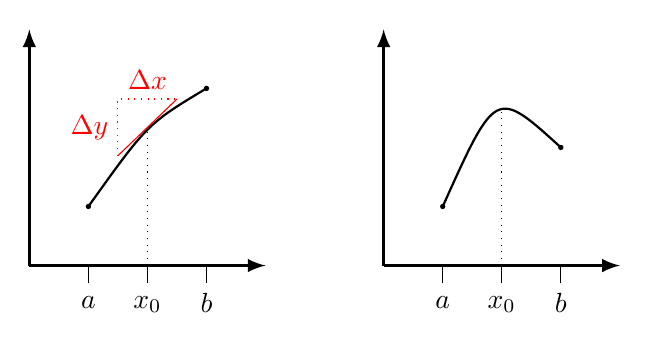
\begin{tikzpicture}[scale=1.5]
        \draw[very thick, -latex] (0, 0) -- (0, 2);
        \draw[very thick, -latex] (0, 0) -- (2, 0);
        \draw[very thick, -latex] (3, 0) -- (3, 2);
        \draw[very thick, -latex] (3, 0) -- (5, 0);
        \draw[] (0.5, 0) -- (0.5, -0.15);
        \node[below] at (0.5, -0.18) {$a$};
        \draw[] (1, 0) -- (1, -0.15);
        \node[below] at (1, -0.18) {$x_0$};
        \draw[] (1.5, 0) -- (1.5, -0.15);
        \node[below] at (1.5, -0.15) {$b$};
        \draw[] (3.5, 0) -- (3.5, -0.15);
        \node[below] at (3.5, -0.18) {$a$};
        \draw[] (4, 0) -- (4, -0.15);
        \node[below] at (4, -0.18) {$x_0$};
        \draw[] (4.5, 0) -- (4.5, -0.15);
        \node[below] at (4.5, -0.15) {$b$};
        \draw[thick] (0.5, 0.5) .. controls(1, 1.2) .. (1.5, 1.5);
        \filldraw[] (0.5, 0.5) circle (0.5pt);
        \filldraw[] (1.5, 1.5) circle (0.5pt);
        \draw[dotted] (1, 0) -- (1, 1.15);
        \draw[red] (0.75, 0.93) -- (1, 1.17) -- (1.25, 1.41);
        \draw[dotted, red] (0.75, 0.93) -- (0.75, 1.41) -- (1.25, 1.41);
        \node[left, text = red] at (0.75, 1.17) {$\Delta y$};
        \node[above, text = red] at (1, 1.41) {$\Delta x$};
        \draw[thick] (3.5, 0.5) .. controls(3.95, 1.5) .. (4.5, 1);
        \filldraw[] (3.5, 0.5) circle (0.5pt);
        \filldraw[] (4.5, 1) circle (0.5pt);
        \draw[dotted] (4, 0) -- (4, 1.3);
        \end{tikzpicture}
    
    \caption{Example demonstrating the above theorem. For the left function, we have that $g = f^{-1}$ exists, and $g'(f(x_0)) = \frac{1}{f'(x_0)} = \frac{1}{\frac{\Delta y}{\Delta x}} = \frac{\Delta x}{\Delta y}$. For the left function, we have that $f'(x_0) = 0$, so no inverse exists near this point (the inverse does not exist on $(x_0 - \e, x_0 + \e)$ for some $\e$).}
    \label{fig63}
\end{figure}

\setcounter{rudin}{23}
\begin{theorem}{The Inverse Function Theorem}{9.24}
    Suppose $\v{f}: E \mapsto \RR^n$ where $E \subset \RR^n$ is open. Suppose $\v{f} \in C^1(E)$, $\v{a} \in E$, and $\v{f}'(\v{a})$ is invertible (c.f. $f'(a) \neq 0$ for the $n = 1$ case). Let $\v{b} = \v{f}(\v{a})$. Then:
    \begin{enumerate}[label = (\arabic*)]
        \item There exists an open set $U, V$ with $\v{a} \in U, \v{b} \in V$ such that $\v{f}: U \mapsto V$ is a bijection. Hence, the inverse function $\v{g} = \v{f}^{-1}$ exists with $\v{g}: V \mapsto U$ and $\v{g}(\v{f}(\v{x})) = \v{x}$ for all $\v{x} \in U$.
        \item $\v{g} \in C^1(V)$.
    \end{enumerate}
\end{theorem}
\noindent Note in the above theorem that both the domain and codomain are $n$-dimensional; the dimensions must match for an inverse to exist (there would be no inverse for $f: \RR^2 \mapsto \RR$, for example). Now, a couple more remarks before we move onto the proof.
\begin{enumerate}[label = \alph*)]
    \item By the chain rule, we have that $\v{g}'(\v{f}(\v{x}))\v{f}'(x) = I$, so $\v{g}'(\v{f}(\v{x})) = \left(\v{f}'(\v{x})\right)^{-1}$ for $\v{x} \in U$.
    \item Let us write $\v{y} = \v{f}(\v{x})$ as $\v{y} = (y_1, \ldots, y_n)$ where $y_1 = f_1(x_1, \ldots, x_n)$, $y_2 = f_2(x_1, \ldots, x_n)$ and so on (up to $y_n = f_n(x_1, \ldots x_n)$). Note that $f_1, \ldots f_n$ could (in general) be horrible nonlinear functions. Writing $\v{y}$ in this way, we generate a system of equations. In math, we are often interested in whether a system of equations is solvable. If $\v{f}'(\v{a})$ is indeed invertible, then for $\v{y}$ near $\v{b} = \v{f}'(\v{a})$, there exists a unique $C^1$ solution $x_1 = g_1(y_1, \ldots y_n), x_2 = g_2(y_1, \ldots, y_n), \ldots, x_n = g_n(y_1, \ldots, y_n)$. $\v{f}$ is a bijection from $U \mapsto V$, and hence there is an inverse function that gives a unique solution $\v{x}$ to any $\v{y}$. And this function is continuously differentiable!
    \item $\v{f} \in C^1$ is assumed. So, the invertibility of $\v{f}'(\v{a})$ is equivalent to the determinant of the matrix representation of the linear operator being non-zero:
    \begin{align*}
        J\v{f}(\v{a}) = \det\m{\dpd{f_1}{x_1}(\v{x}) & \cdots & \dpd{f_n}{x_1}(\v{x})
        \\ \vdots & \ddots & \vdots
        \\ \dpd{f_1}{x_n}(\v{x}) & \cdots & \dpd{f_n}{x_n}(\v{x})} \neq 0
    \end{align*}
    this is because $\v{f}'(\v{a})$ being invertible if and only if the matrix representation is invertible if and only if the matrix representation has nonzero determiant. This determinant is known as the \emph{Jacobian determinant} of $\v{f}$ at $\v{a}$. 
\end{enumerate}

\begin{nblank}{Proof of (1)}
    For the first step, we show that there exists open $U \ni \v{a}$ such that $\v{f}$ is one-to-one on $U$. Write $A = \v{f}'(\v{a})$. We will now used the Banach fixed point theorem/Theorem \ref{thm:9.23} (Note: This requires some ingenuity). Given $\v{y} \in \RR^n$, let $\gv{\phi}(\v{x}) = \v{x} + A^{-1}(\v{y} - \v{f}(\v{x}))$ (note that $\gv{\phi}$ depends on $\v{y}$). Then, $\gv{\phi} = \v{x}$ if and only if $\v{y} = \v{f}(\v{x})$ (as $A^{-1}\v{z} = 0$ if and only if $\v{z} = \v{0}$). Hence, the uniqueness of the fixed point of $\gv{\phi}$ implies a fixed point of $\v{x}$ such that $\v{y} = \v{f}(\v{x})$, which is the claim. It therefore suffices to show that $\gv{\phi}$ is a contraction. We will demonstrate this via the derivative. We have that $\gv{\phi}'(\v{x}) = I - A^{-1}\v{f}'(\v{x})$. We can factor out $A^{-1}$ to write $\gv{\phi}'(\v{x}) = A^{-1}(\v{f}'(\v{a}) - \v{f}'(\v{x}))$. We therefore have that $\norm{\gv{\phi}'(\v{x})} \leq \norm{A^{-1}}\norm{\v{f}'(\v{a}) - \v{f}'(\v{x})}$. Since $\v{f}'$ is continuous, there exists $\delta > 0$ such that $\norm{\v{f}'(\v{a}) - \v{f}'(\v{x})} \leq \frac{1}{2\norm{A^{-1}}}$ if $\abs{x - a} < \delta$. Hence, $\norm{\gv{\phi}'(\v{x})} \leq \frac{1}{2}$ if $\v{x} \in N(\v{a})$ which identifies the desired set $U$. For $\v{x}_1, \v{x}_2 \in U$, we have that $\abs{\gv{\phi}(\v{x}_1) - \gv{\phi}(\v{x}_2)} \leq \frac{1}{2}\abs{\v{x}_1 - \v{x}_2}$ by Theorem \ref{thm:9.19}. So, $\gv{\phi}$ is a contraction of $U$, and hence $\gv{\phi}$ has at most one fixed point. Therefore, $\v{f}$ is one-to-one on $U$.

    Fo the second step, let $V = \v{f}(U)$. We show that $V$ is open (as this proves (1)). Let $\v{y}_0 \in V$, say, $\v{y}_0 = \v{f}(\v{x}_0)$ ($\v{x}_0 \in U$). We need to find $\e > 0$ such that $N_\e(\v{y}_0) \subset V$, i.e. for every $\v{y} \in N_\e(\v{y}_0)$, there exists $\v{x} \in U$ such that $\v{f}(\v{x}) = \v{y}$. Given $\v{y} \in \RR^n$, as before, define $\gv{\phi}_\v{y}: \RR^n \mapsto \RR^n$ by $\gv{\phi}_{\v{y}}(\v{x}) = \v{x} + A^{-1}(\v{y} - \v{f}(\v{x}))$ (with $\v{x} \in U$). Note that this neighbourhood of $U$ is \emph{not} complete (unless it happens to be all of $\RR^n$). Next, choose $r > 0$ such that $\overline{B} = N_r(\v{x}_0) \subset U$ which is possible as $U$ is open. For $\v{x} \in \overline{B}$, we show that $\abs{\gv{\phi}_\v{y}(\v{x}) - \v{x}_0} < r$. For this, we observe that:
    \begin{align*}
        \abs{\gv{\phi}_{\v{y}}(\v{x}) - \v{x}_0} \leq \abs{\gv{\phi}_{\v{y}}(\v{x}) - \gv{\phi}_{\v{y}}(\v{x}_0)} + \abs{\gv{\phi}_{\v{y}}(\v{x}_0) - \v{x}_0}
        &\leq \frac{1}{2}\abs{\v{x} - \v{x}_0} + \abs{\v{x}_0 + A^{-1}(\v{y} - \v{f}(\v{x}_0)) - \v{x}_0}
        \\ &= \frac{1}{2}\abs{\v{x} - \v{x}_0} + \abs{A^{-1}(\v{y} - \v{f}(\v{x}_0))}
        \\ &\leq \frac{1}{2}\abs{\v{x} - \v{x}_0} + \norm{A^{-1}}\abs{\v{y} - \v{f}(\v{x}_0)}
        \\ &= \frac{1}{2}\abs{\v{x} - \v{x}_0} + \norm{A^{-1}}\abs{\v{y} - \v{y}_0}
    \end{align*}
    We choose $\e = \frac{r}{2\norm{A^{-1}}} < \frac{1}{2}r + \norm{A^{-1}}\frac{r}{2\norm{A^{-1}}}$. Therefore, $\gv{\phi}_{\v{y}}(\v{x}) \in \overline{B}$, that is, $\gv{\phi}_{\v{y}}: \overline{B} \mapsto \overline{B}$. We know from step 1 that $\gv{\phi}_{\v{y}}$ is a contraction on $\overline{B}$, and $\overline{B}$ is complete, so by the fixed point theorem/Theorem \ref{thm:9.23}, there exist a unique fixed point $\v{x} \in B \subset U$ such that $\gv{\phi}_{\v{y}}(\v{x}) = \v{x}$. This $\v{x}$ obeys $\v{y} = \v{f}(\v{x})$ so $\v{y} \in V$. \qed
\end{nblank}

\noindent As a remark, note that coming up with $\gv{\phi}$ in the above first part of the proof is quite difficult/inspired; this is definitely not a simple proof to come up with! After this first part, we have shown the existence of an open $U \ni \v{a}$ such that $\v{f}: U \mapsto V$ is a bijection. Note that we need $V$ to be open for the proof of the second part of the theorem, as we need the derivative (which we only defined on open sets) to make sense.

\begin{nblank}{Proof of (2)}
    We show that $\v{g} = \v{f}^{-1}: V \mapsto U$ is in $C^1(V)$. Let $\v{y} \in V$. Then, $\v{y} = \v{f}(\v{x})$ sor some unique $\v{x}$. Since $U$ is open, take $\v{k}$ small enough such that $\v{y} + \v{k} \in V$. Say, $\v{y} + \v{k} = f(\v{x}_{\v{k}})$ where $\v{x}_{\v{K}} \in U$. Let $S = \v{f}'(\v{x})$ and $T = S^{-1}$. Note that $(\v{f}'(\v{x}))^{-1}$ exists by a continuity argument ($\v{f}'(\v{x})$ is close to $\v{f}'(\v{a})$ and $\v{f}'(\v{a})$ is invertible; see Rudin 9.8). Consider the expression:
    \begin{align*}
        \frac{\abs{\v{g}(\v{y} + \v{k}) - \v{g}(\v{y}) - T(\v{k})}}{\abs{\v{k}}}.
    \end{align*}
    We want to show that this goes to zero as $\v{k} \rightarrow \v{0}$. The idea is that somehow, we will turn this ratio into the derivative of $\v{f}$. Doing some algebra, we have that:
    \begin{align*}
        \v{g}(\v{y} + \v{k}) - \v{g}(\v{y}) - T(\v{k}) = \v{g}(\v{f}(\v{x}_{\v{k}})) - \v{g}(\v{f}(\v{y})) - T\v{k} &= \v{x}_{\v{k}} - \v{x} - T\v{k} 
        \\ &= -T\left((\v{f}(\v{x}_{\v{k}}) - \v{f}(\v{x})) - S(\v{x}_{\v{k}} - \v{x})\right)
    \end{align*}
    Taking the norm of both sides, we have:
    \begin{align*}
        \abs{\v{g}(\v{y} + \v{k}) - \v{g}(\v{y}) - T(\v{k})} \leq \norm{T}\abs{\v{f}(\v{x}_{\v{k}}) - \v{f}(\v{x}) - S(\v{x}_{\v{k}} - \v{x})}
    \end{align*}
    Note that $\v{f}(\v{x}_{\v{k}}) - \v{f}(\v{x}) = \v{k}$. Also, we want to prove $\abs{\v{x}_\v{k} - \v{x}} \leq 2\norm{A^{-1}}\abs{\v{k}}$. Next, we have that:
    \begin{align*}
        \gv{\phi}_\v{y}(\v{x}_\v{k}) - \gv{\phi}_\v{y}(\v{x}) = \v{x}_\v{k} - \v{x} + A^{-1}(\v{f}(\v{x}) - \v{f}(\v{x}_\v{k}))
    \end{align*}
    So therefore:
    \begin{align*}
        \v{x}_\v{k} - \v{x} = \gv{\phi}_\v{y} - \gv{\phi}_\v{y} + A^{-1}\v{k} \implies \abs{\v{x}_\v{k} - \v{x}} &\leq \abs{\gv{\phi}_\v{y} - \gv{\phi}_\v{y}} + \norm{A^{-1}}\abs{\v{k}}
        \\ &\leq \frac{1}{2}\abs{\v{x}_\v{k} - \v{x}} + \norm{A^{-1}}\abs{\v{k}}
    \end{align*}
    where in the last inequality we use the result from step 1 of the proof ($\gv{\phi}$ is a contraction with constant $\frac{1}{2}$). From this, we obtauin that $\abs{\v{x}_\v{k} - \v{x}} \leq 2\norm{A^{-1}}\abs{\v{k}}$ (as we wanted!) and hence $\frac{1}{\abs{\v{k}}} \leq \frac{2\norm{A^{-1}}}{\abs{\v{x}_\v{k} - \v{x}}}$.We therefore have that:
    \begin{align*}
        \abs{\v{g}(\v{y} + \v{k}) - \v{g}(\v{y}) - T\v{k}} &\leq \frac{2\norm{A^{-1}}}{\abs{\v{x}_\v{k} - \v{x}}}\norm{T}\abs{\v{f}(\v{x}_\v{k}) - \v{f}(\v{x}) - S(\v{x}_\v{k} - \v{x})} 
        \\ &= 2\norm{A^{-1}}\norm{T}\frac{\abs{\v{f}(\v{x}_\v{k}) - \v{f}(\v{x}) - S(\v{x}_\v{k} - \v{x})}}{\abs{\v{x}_\v{k} - \v{x}}}
    \end{align*}
    Now, let $\v{k} \rightarrow \v{0}$. Then, $\v{x}_\v{k} - \v{x} \rightarrow \v{0}$, so the RHS goes to $0$ as $S$ is $\v{f}'$ and hence this is just the definition of the derivative. Continuity follows from the fact that when you move an operator in a continuous way, so too does its image. \qed
\end{nblank}
\begin{center}
    \textbf{THE END}
\end{center}